\subsection{Manipulacion}

\begin{figure}[H]
\centering
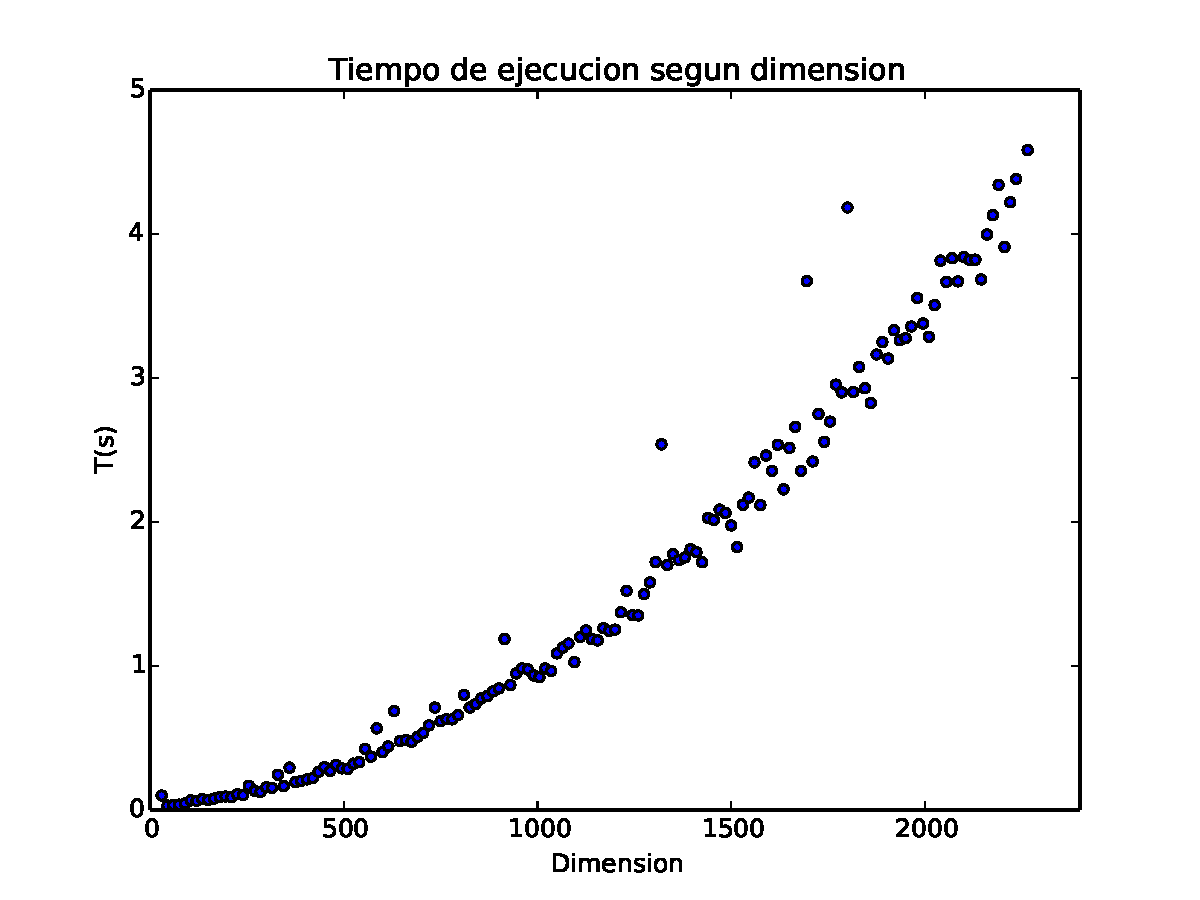
\includegraphics[scale=0.7]{images/complejidad.pdf}
\caption{Tiempos de ejecución según cantidad de webs.}
\label{timePageRank}
\end{figure}




página 5, ejercicio 1. La idea es que plantees un caso de un tipo que quiere manipular el ranking, mostra que aunque agregues miles de nuevas páginas apuntando no podes hacer demasiado, hacelo en funcion de la cantidad de páginas que agregas?

Se puede manipular entonces o no? Agarra, en el eje x pone cantidad de sitios web que apuntan solamente al sitio u que le quiero subir el ranking, y en el eje y el ranking de ese sitio. Fijate que aumenta, y fijate si podes hacer algun tipo de curva de nivel con c (cuanto mayor c, mas manipulable es la cosa). Citar el paper de Sergei y Brin, que dicen que hacen promedios de muchas cosas en la practica para evitar este problema. Usan muchos criterios promediados.